\subsubsection*{Cost Category 22.01.07: Power Supplies} 

This category covers an extensive range of power supply systems critical for operation. This includes High-Voltage Power Supplies for plasma heating, Pulsed Power Supply Systems for plasma initiation, and Superconducting Coil Power Supplies for magnetic confinement. Auxiliary Heating Power Supplies support additional plasma heating, while Cooling and Cryogenic Systems maintain optimal temperatures for superconducting components. 


\begin{itemize}
    \item Cost Category 22.07.01 High-Voltage Power Supplies. Essential for driving heating systems like neutral beam injectors, which heat the plasma to the necessary temperatures for fusion.
    \item Cost Category 22.07.02 Pulsed Power Supply Systems. These provide high-power electrical pulses required for plasma initiation and shaping.  This is the dominant cost category here.  We have built 0.5MJ, 20kV, 500kA capacitor banks for 200k USD each, we multiply by 15 to get to the 6MJ needed for each pulse, and operate at 5kV to get lifetime needed for life of plant (see Fig. \ref{fig:derate}).  We further multiply the number of banks we need by 5 to get the charge timing.  Cost of this element is \$ C220702 M.


    \item Cost Category 22.07.03 Coil Power Supplies: These are crucial for large superconducting magnets, and copper coils for equilibrium control.
    \item Cost Category 22.07.04 Auxiliary Heating Power Supplies. These are used for additional plasma heating systems like ion cyclotron resonance heating (ICRH) and electron cyclotron resonance heating (ECRH).
    \item Cost Category 22.07.05 Cooling and Cryogenic Systems. To maintain the necessary low temperatures for the superconducting magnets and other components.
    \item Cost Category 22.07.06 Control and Instrumentation Power Supplies. For the myriad of sensors, diagnostics, and control systems involved in monitoring and controlling the fusion reactor.
    \item Cost Category 22.07.07 Power Conversion Systems for Plasma Heating. Such as gyrotrons for ECRH and klystrons or tetrodes for ICRH.
    \item Cost Category 22.07.08 Safety and Interlock Systems. To ensure safe operations, especially during abnormal events or emergencies, these systems can cut power or initiate shutdown sequences.
    \item Cost Category  22.07.09 Diagnostics and Monitoring Systems Power Supply. For real-time monitoring of plasma and reactor conditions, requiring reliable and clean power sources.
\end{itemize}

%need to escalate this cost relative to the 2011 data from ITER:
%https://docs.google.com/spreadsheets/d/1MHiUnJ580Vxzbb7P5V9vQH0PnGHsuDlx/edit?usp=sharing&ouid=106425516412438351916&rtpof=true&sd=true
%Cost basis is taken from ITER for a 500MW fusion system, scaling the 269.6kIUA (1kIUA is 2MUSD), giving 539M USD for a 500MW fusion system. 

This system is costed in two main parts: a calculation of the power requirements and cost based on the details of the confinement system, and a top-down costing for the full electrical power supply and distribution system, scaled from ITER. For this external infrastructure required for ITER, a 500 MW fusion system, the total cost was 269.6kIUA or 539M USD. 
We expect these FOAK costs to follow a usual learning curve for NOAK, and so apply an 80\% learning curve credit to the ITER cost. Thus, with the bottom-up component for the compression system, and the top-down component for external infrastructure, the total cost is found: for compression system power supplies, the cost is \$ C22010701 M, and \$ C22010702 M for the full electrical power supply and distribution system. 

The total cost is therefore C220107 M USD for the PNRL MW fusion system presented here. 

\begin{figure}[h!]
    \centering
    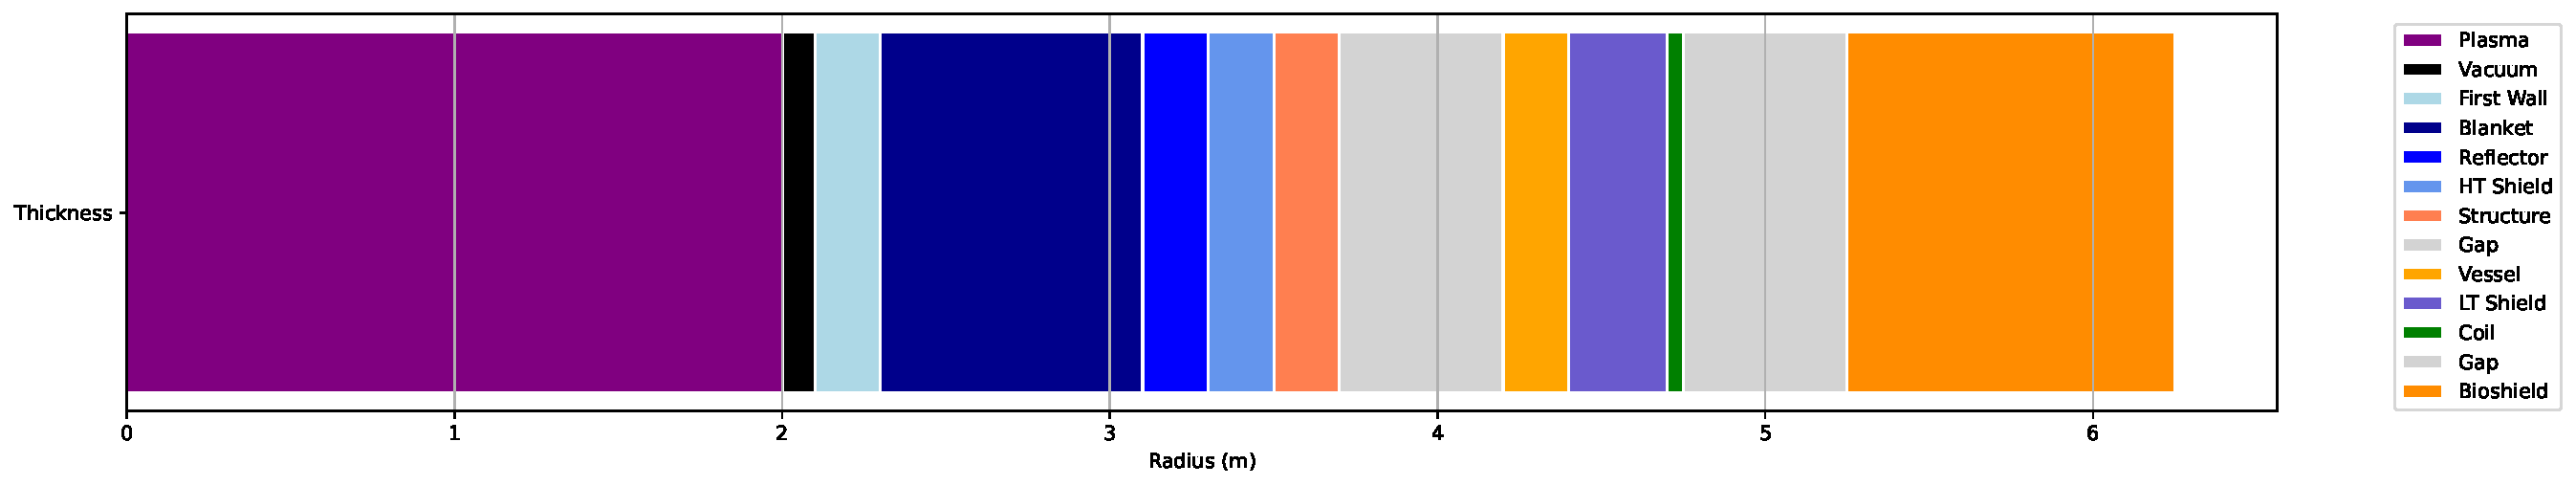
\includegraphics[scale=0.4]{Figures/cap_derate.pdf}
    \caption{Lifetime extension factor vs ratio of applied to rated voltage.}
    \label{fig:derate}
\end{figure}



